\documentclass{article}

\usepackage{graphicx}
\graphicspath{ {./images/} }

\usepackage{tikz}
\usetikzlibrary{shapes.geometric, arrows} 
\usepackage{hyperref}
\hypersetup{
    colorlinks=true,
    linkcolor=blue,
    filecolor=magenta,      
    urlcolor=cyan,
    pdftitle={Overleaf Example},
    pdfpagemode=FullScreen,
}
\usepackage{titlesec}
\usepackage{geometry}
 \geometry{
 a4paper,
 total={170mm,257mm},
 left=20mm,
 top=20mm,
 }

%flowchart
\tikzstyle{startstop} = [rectangle, rounded corners, minimum width=3cm, minimum height=1cm, text centered, draw=black, fill=red!30]
\tikzstyle{io} = [trapezium, trapezium left angle=70, trapezium right angle=110, minimum width=3cm, minimum height=1cm, text centered, draw=black, fill=blue!30]
\tikzstyle{process} = [rectangle, minimum width=3cm, minimum height=1cm, text centered, draw=black, fill=orange!30]
\tikzstyle{decision} = [diamond, minimum width=3cm, minimum height=1cm, text centered, draw=black, fill=green!30]
\tikzstyle{arrow} = [thick,->,>=stealth]

\title{Unit 15 LO2}
\author{Chris}
\date{}

\begin{document}

\maketitle
\tableofcontents
\break

\section{P3 Create a design for an identified game concept}
We have been tasked in the previous Units to create a game for a food retailer. They are a fresh and modern company who are aware of moderen digital marketing techniques.
They are clear that they want to have a game developed which will be used as a part of their advertising campaigns. To that end they want to have a game developed that incorporates their branding and mascot, a food ninja.
The artifacts in the game must relate to their fast food outlets and the gameplay must be fun and engaging and reflect their healthy attitudes to food. 

The game is to be targetted at a younger audience and should have a an easy to pickup layout, meaning that the game play should be something most players will have played previously. To that end a platformer has been requested. 

\subsection{Game elements}
\subsubsection{Navigation}
The navigation in the game is done by providing important information to the player to the player by either using a Heads Up Display(HUD) for example compasses,maps or arrow signs. Both of these methods are helpful in games and their use depends on game's genre and how the game designers want the player to experience the game.

The HUD said by Greg Wilson in the article \textit{Off With Their HUDs} described HUD as "A collection of persistent onscreen elements whose purpose is to indicate player status. HUD elements can be use to show, among many other things, how much health the player has, in which direction the player is heading, or where the player ranks in a race" 



\subsubsection{Scoring}
Scoring in games are key component of game mechanics and it provides a mechanic where the players get rewarded with point value whenever they accomplish a task in the game.   
In this game the scoring will be based upon the collection of sweets that our client, the food producer creates. Thier mascot, a ninja will run swideways on the platformer and will need to avoid or defeat various monsters to be able to continue. As the ninja continues to move they will encounter various sweets that will increase their score, some of these sweets will also be dropped by the monsters which have been killed.

\subsubsection{Movement}
Moving a character is so common in games that players and designers often take it for granted. However, while it can be tempting to use the default movement options in a game engine, designing great movement can make simply controlling a character fun. 
Movement of the character in this game should be verty straightfoward, as this is a traditional 2D platformer the main character will need to
\begin{itemize}
\item Move left
\item Move right
\item Jump
\item Duck / Hide
\end{itemize}

It would be easy to add other actions such as adding combos that build up actions like Mortal Kombat or Super Smash Brothers but as the remit for this game is something which is familar we will stick with the basic movements for the first demo to the customer.

The controls will also default to the standard WASD controls but we will add a configuration page so that users can remap the controls if they want to.

\subsubsection{Interaction/Controls}
three main principles for good game controls are:
\begin{itemize}
	\item Accessibility - the controls should be easy to learn and use, and take into account physical and cognitive limitations
	\item Intent Communication - the controls should communicate the player's intent in a way the player expects and create a feeling of full control
	\item Expression Space - the controls should give the player enough expression so that they players can master while also keep a sufficient level of variety.
\end{itemize}

Accessibility 
If we want our controls to be easy to learn and use we need to take into account everyone physical and cognitive limitation 

\subsubsection{Conveying Information}
Classic tutorials are one of the worst ways to convey information to the players about the game. These levels are are often some of the least fun parts of the entire game and some are un-skippable these are worst, making them not every effective at their job.

\subsubsection{Sound}
Designing Sounds in a game are:
Talking about various sounds found in a particular game, those could be generalised to the following types: 
\begin{itemize}
	\item Sound Effects - The sounds the objects in the game game make
	\item Music -  A game has 2 or 3 main themes for example menu music and the level music
	\item Voice-overs - are the character lines
\end{itemize}

\subsubsection{Levels}
Their will be 5 levels in our game and all of them are going to themed after our clients food. Each level is unique and different from each other 

\subsubsection{Enemies}
The eniemes of the game will be small and easy to hit since this game is designed for kids and young teens. The height of these mobs will be half height of the player character. We do this because it makes it easier for our target audience to understand our game and theconcepts to the gamer. 


\subsubsection{Problem Solving}
The is small amount of problem solving in our game because we are 2D platformer and we have small traps and enemies for the player to get around. The traps are disguised to hide/blend them into scenario so that they "get" the player, the traps do look different enough that the players can detect and dodge the traps.

\subsection{Interface Design}
\subsubsection{layout}
The Layout out of each levels is going to be designed to promoted a 

\subsubsection{Colour Palette}
The colour palette is going to be bright eye catching colours for the  

\subsubsection{Text Styles}
The text style for the game is going to cartoony style to entise our target audience to click and download our clients game. 

\subsubsection{Sound}
The sound for the game is basic as can be and will be kept to minium since they are uneccessery and execpt the game to be muted when playing since it will be on a phone

\subsubsection{Stage/Scene}
Stage in the game is going ot simplre and 

\subsubsection{Actions}
Actions that will be done are fighting enimes and 


\section{P4 Produce a logic structure for the identified game concept}
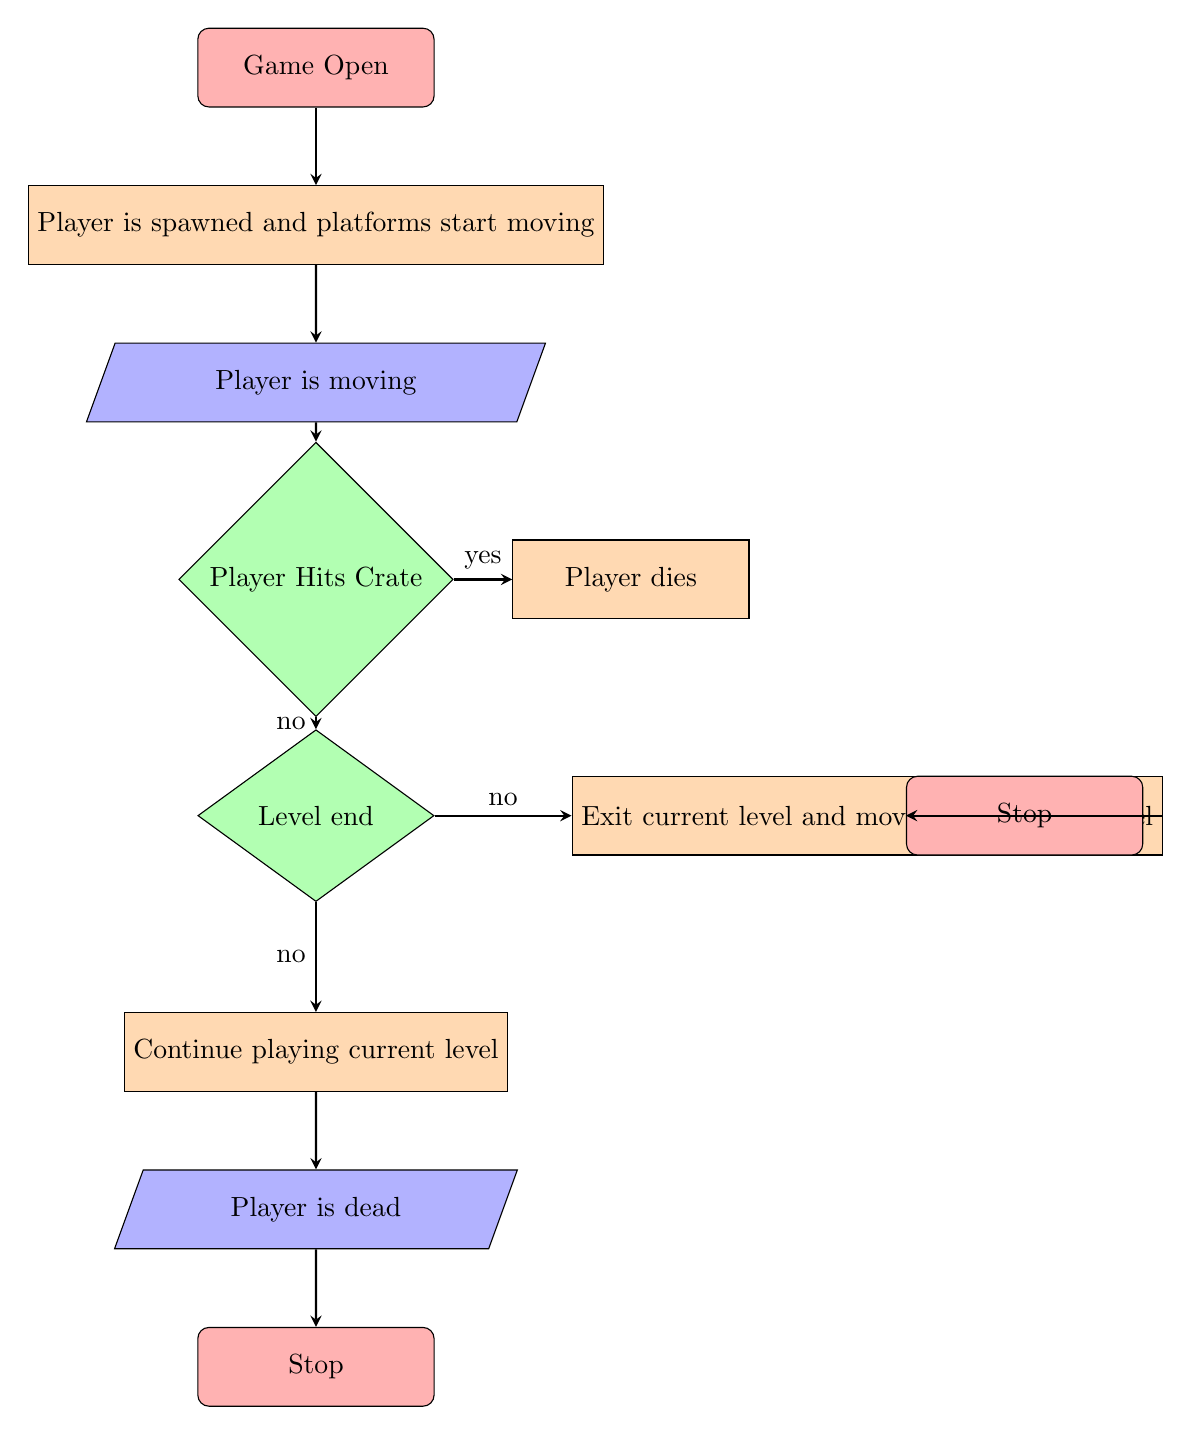
\begin{tikzpicture}[node distance=2cm]
	\node (start) [startstop] {Game Open};
	\node (proc1) [process, below of=start] {Player is spawned and platforms start moving};
		\draw [arrow] (start) -- (proc1);
	\node (in1) [io, below of=proc1] {Player is moving};
		\draw [arrow] (proc1) -- (in1);
		
	\node (dec1) [decision, below of=in1, yshift=-0.5cm] {Player Hits Crate};
		\draw [arrow] (in1) -- (dec1);
		
	\node (proc2b) [process, right of=dec1, xshift=2cm] {Player dies};
		\draw [arrow] (dec1) -- node[anchor=south] {yes} (proc2b);
		
	\node (dec2) [decision, below of=dec1, yshift=-1cm] {Level end};
		\draw [arrow] (dec1) -- node[anchor=east] {no} (dec2);
	\node (proc3b) [process, below of=dec2, yshift=-1cm] {Continue playing current level};
		\draw [arrow] (dec2) -- node[anchor=east] {no} (proc3b);
			
	\node (proc3a) [process, right of=dec2, xshift=5cm] {Exit current level and move onto the next level};
		\draw [arrow] (dec2) -- node[anchor=south] {no} (proc3a);
	\node (stop1) [startstop, right of=proc3a] {Stop};
		\draw [arrow] (proc3a) -- (stop1);

	\node (out1) [io, below of=proc3b] {Player is dead};
		\draw [arrow] (proc3b) -- (out1);
	\node (stop2) [startstop, below of=out1] {Stop};
		\draw [arrow] (out1) -- (stop2);
	
\end{tikzpicture}




\section{M2 Prepare alternative interface designs for the identified game concept}
Alternative interface designs is a hudless design. This done by having these elements integrated into the world for the health,score and timers. 
The hud can be easily show in the game world by having visual signs to the user, this can be done by having a bars or having the player character getting more visually hurt.
The score system can be shown either by having the players outfit or having a glow around the player character to indicate the score is increasing. The former we think is the best because it immediately rewards the player and makes the player want to get higher score since the player will look better the more points they get 
The time can either be done by sound or having and effect on the player makes the player feel dread and cause the player hury up and finish the levels. The ladder is the best option because it cause more dread for the player and we don't think this will make our young audience scared of our game

If our client want to get rid of the hud and seemless interface between the game and the user, having no hud is one of the way this makes of getting the player immersed into game. Getting immersion in game is hard but having no hud can easily increase the immersion a player can have.



Prepare alternative interface designs to the one identified in P3. The alternative designs must contain enough detail to enable them to be understood by a third party. Evidence can be extension of P3 and be presented as additional visualisations or written explanatory designs, or a combination of both.


\subsection{ Sprites Looks and Feel }
As we are developing a 2D platformer, we want to keep with a retro theme. We have an option to be authentic to 80s sprites, which would mean keeping the edges sharp, using a much smaller colour palette and the resolution would be low.
This is somewhat tempting as it would look like it would be keeping with the theme of making the game look familiar, but when you actually look at any examples of sprites from that era, they tend to look what can only be described as low-res and rough.

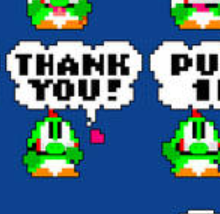
\includegraphics[scale=0.5]{TraditionalSprite}

As retro games became more popular, over the last decade or so, a sort of hybrid of old and new styles have become more popular, and in keeping with the remit of developing something which is familar, we are going to go with the more modern retro look sprites.

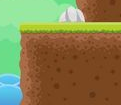
\includegraphics[scale=0.5]{SoftSprite}


\section{D1 Justify the design rational for the identified game concept}


\subsection{Original requirements}
To justify the design choices in our game we must first explicitly spell out the requirements as they were given to us

\begin{itemize}
\item The whole game experience must be familiar and easy to get to understand
\item The UX must not be confusing
\item Must work on all devices
\item Must be appealing to a younger audience
\item Players must have seen the likes of the game before
\item It must be small in scale, there will only be five levels
\item It must be engaging
\item It will have the clients food products
\item It will have monsters that must be defeated
\item It will educate players about the variety of foods, highlighting their unique qualities
\item Health boosts should be in the game based on their food products
\item As the player progresses through the levels, each level will become harder
\item There will be obstacles in the players way which must an navigated around. These should present moderately hard puzzles
\item On completion of the game the player is rewarded with a lifetime supply of the client's food
\end{itemize}

We will work through these one at a time

\subsection{ The whole game experience must be familiar and easy to get to understand }
This requirement is probably the one that has the largest impact on the game. It has made the design of the game a lot easier and quicker to develop as it has restricted us from try to deisgn a modern AAA game and instead we have been able to take a much more retro approach to designing the game. The logic behind this has been that as games from an earlier age of video games has been around a long time and almost everyone will have experienced these style of games in one form or another. 
This left the decsion as to which style of retro game to use. Games like Space Invaders and Pong, while they are arguably the grandfather of all modern games, they are not so well known in modern times and their gameplay mechanics is likely less understandable to a younger generation. Games of that era tended to be a bit more archiac. 
Moving on to games such a Pacman, Frogger, etc are also more well known but are a little too simplistic to provide an engaging and interesting gameplay.
Slightly more modern games such as Super Mario Brothers are much more well known and understood without have to have any preamble to explain what is happening. It was felt that it was too tempting to make this game as universal as it could be by using a side scrolling 2D platformer, so this is what we decided to go for. It not only means that it will be familiar, but there will also be very little friction for users starting to play the game. We will need to play test the game at an early stage with younger audiences but we are confident that they will have no problems understanding the mechanics.
 
\subsection{ The UX must not be confusing }
Making the user interface experience not be confusing also partially ties in to the requirement that the game must be familiar. It however goes furhter than that. We have decdided to use standard controls, as these are well known and very simple it means that this part of the game should be intuitive.
2D platforms usually have a retro 'language' or 'theme'. They are usually blocky but not blocky in the way that 80s sprites would have been but more blockly in the same sort of style as Minecraft, with softer edges and corners. This was one of the considerations in M2, should the sprites look hard oor soft. The harder version of sprites are not very popular and would likely put players off, so we went with a more fashionable softer look.

\subsection{ Must work on all devices }
This requirment is self evident in todays market. As most players / clients will be accessing the internet on many different devices, we are left with no other option than to ensure that our game will at the very least work on the major devices.
The mobile market has become the dominant device when it comes to accessing the internet, though the lowly PC is still not far behind \url{https://gs.statcounter.com/platform-market-share/desktop-mobile-tablet}

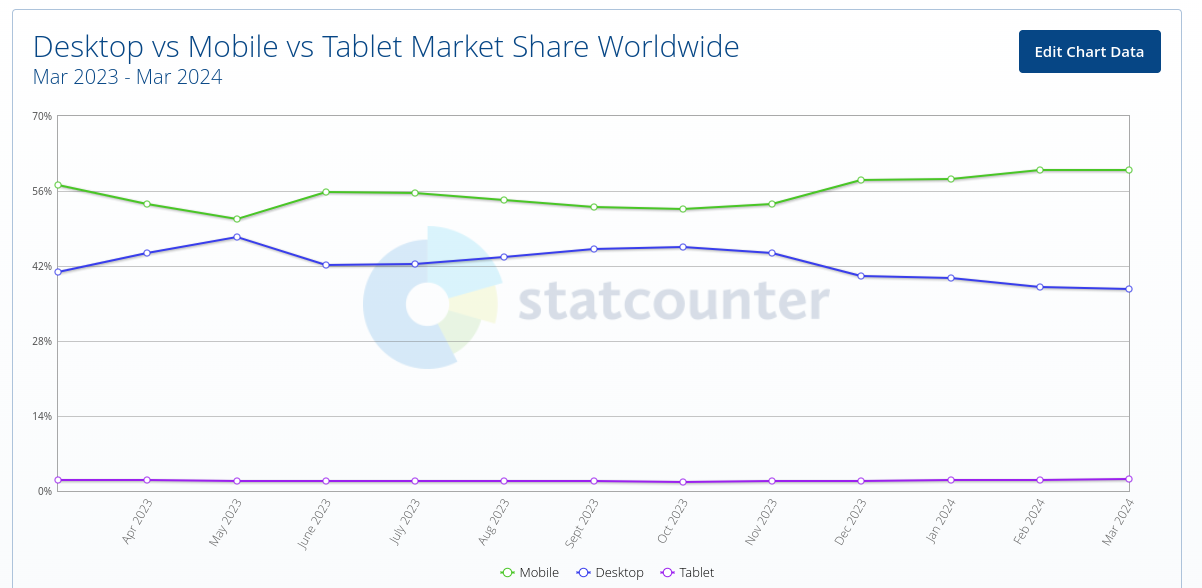
\includegraphics[scale=0.35]{MobileVsPC}

This means we will have to develop for multiple platoforms. This may mean relying on a games engine or developing everything natively. Either way we will need to test on all relevant platforms, and on multiple mobile phones and PC browsers, to make sure that the majority of customers have a good experience. This will not be cheap but the alternative is a bad experience for a lot of customers.

\subsection{ Must be appealing to a younger audience }
\subsection{ Players must have seen the likes of the game before }
The requirement that the game must be appealing to a younger audience was driven by the client, this is something that has tied in to what our sprite look like and the conecpt that it must be easy to pickup and play the game.
We are not able top make the assumption that younger game players will have experience with older 2D platformer mechanics, so we have had to investigate the character handling in the likes of Minecraft and more recent Mario games. It turns out that the basic concept of moving in one direction by pressing one key is pretty universal. A key for jumping also seems universal as well so it would seem that we can make assumptions on how to control the character.
The game play of going from a starting point to and end point and then starting a new level is ubiquitous in Mario games so we felt that we could rely on this mechanic as Mario and Nintendo are arguably the largest video game company at the moment.

\subsection{ It must be small in scale, there will only be five levels }
It can be very tempting to 'Burn the ocean' as in to try and make a massive world of content that covers everything you or your players can think of. As a part of our remit we were given the opposite requirement, our client wanted us to keep the game small. Their reasoning for this was that they wanted to keep the game simple and fun and also for it to load quickly for players.
This meant that we had two requirements. One was that the amount of time to complete the game had to be limited, but also that all the assets had to remain quite small so that the same would start quickly from a clean start on a browser or mobile phone. In keeping with the theme of developing something that was familiar, we went for a side scrolling 2D platformer in the style of the original Mario Bros. This then very heavily lends itself to the concept of levels. Levels have the advantage that it is then possible to record the leve that a user has gotten to in the browser, meaning that the game is a lot more casual and appealing to people who progress in the game but do not want to spend a lot of time in each session so that they can have a breather.

The concept of keeping the game short and only to five levels is not as restricting as first thought. It could also be possible to add in speed runs, which are a popular gaming mode. In this mode the person who can complete the game in the shortest amount of time is the winner. We could keep a high score table of the fastest runs, though this is all speculative.

\subsection{ It must be engaging }
Engaging is a far reaching term. The only real way we can tell if a game is engaging is to play test it. To that end we will be play testing iterations of our game, section by section and gathering all the metrics we can about player satisfaction. This is a deliberate choice as a part of our design decisions. Through extensive development of games we have found that it is impossible to perfectly predict what players will and will not enjoy. In face game play mechanics which we love in house can turn out be a complete flop while the smallest features such as a mini power up can excite users. Play testing allows us to discover the small things that players enjoy and build on those instead of spending all our time developing a game which flops the first time a player tries it out.

\subsection{ It will have the clients food products }
This is a fundamental part of the customers requirements. The use of their food is the cornerstone of this game.
Most importantly the food items need to be seen in a positive way, and not used for negative purposes such as killing monsters or even subtler things such as standing on them to get to a higher stage as standing on food could be seen as unhygenic. 
The main aim of the game is to get to the end with the highest possible score. As gaining score is the desired positive outcome we then decided that the collection of the customer's food is what would increase your score.

\subsection{ It will have monsters that must be defeated }
A platformer which is a straight race to the end of the level would be very boring. We need to build in some sense of excitement and danger. The easiest and most familar way to do that is to bring in monsters that block your character's way. These monsters could take any form, other ninjas, random objects, blobs, etc. It was felt that we should keep the elements of the game familiar so the design of the monsters was left as small hairy non-descript beings. 
We do not want to introduce the idea that the corporate ninja would fire objects as this could be seen as a negative trait e.g. using projectiles to kill things. Instead we stuck rigidly with the familiar concept of jumping on top of monsters to decapacitate them. Doing this adds an element of risk and skill but does not make the game grotesque.

\subsection{ It will educate players about the variety of foods, highlighting their unique qualities }
This proved to one of the hardest elements to introduce to the game.

\subsection{ Health boosts should be in the game based on their food products }
\subsection{ As the player progresses through the levels, each level will become harder }
\subsection{ There will be obstacles in the players way which must an navigated around. These should present moderately hard puzzles }
Moving platofrm
Falling platofrm
Trap box

\subsection{ On completion of the game the player is rewarded with a lifetime supply of the client's food }

\bibliographystyle{plain}
\bibliography{references}

\end{document}
